\documentclass[11pt, oneside]{article}   	% use "amsart" instead of "article" for AMSLaTeX format
\usepackage{geometry}                		% See geometry.pdf to learn the layout options. There are lots.
\geometry{letterpaper}                   		% ... or a4paper or a5paper or ... 
%\geometry{landscape}                		% Activate for for rotated page geometry
%\usepackage[parfill]{parskip}    		% Activate to begin paragraphs with an empty line rather than an indent
\usepackage{graphicx}				% Use pdf, png, jpg, or eps� with pdflatex; use eps in DVI mode
								% TeX will automatically convert eps --> pdf in pdflatex		
\usepackage{amssymb}
\usepackage{amsmath}
\usepackage{parskip}
\usepackage{color}
\usepackage{hyperref}

\title{Fermat variation}
%\author{The Author}
%\section{}
%\subsection*{}
\date{}							% Activate to display a given date or no date

\graphicspath{{/Users/telliott_admin/Dropbox/Tex/png/}}
% \begin{center} 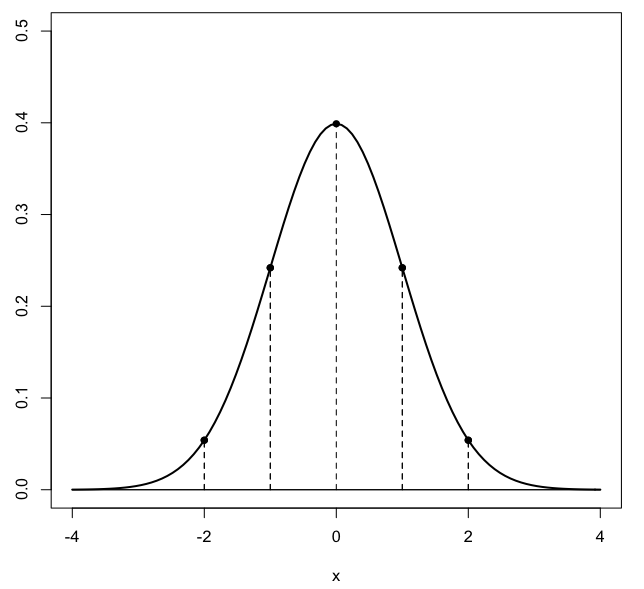
\includegraphics [scale=0.4] {gauss3.png} \end{center}
\begin{document}
\maketitle
\Large
I came across a different way of doing the Riemann sum for the area under the curve of a function $f(x)$ in Maor's \emph{e, the story of a number}.

First, review the standard approach.  We consider the area under the curve $f(x) = x^n$ between $x=0$ and $x=a$.  Divide the interval $[0,a]$ into $k$ rectangles of equal width $a/k$.  The right-hand boundary of each rectangle is 
\[ \frac{a}{k}, \frac{2a}{k}, \frac{3a}{k} \dots \frac{ka}{k} \]
and the value of $f(x)$ at each point is
\[  (\frac{a}{k})^n, (\frac{2a}{k})^n, (\frac{3a}{k})^n \dots (\frac{ka}{k} )^n \]
The width of each interval is $a/k$ so total area is
\[ A = \frac{a}{k} \ [ \ (\frac{a}{k})^n, (\frac{2a}{k})^n, (\frac{3a}{k})^n \dots (\frac{ka}{k} )^n \ ] \]
\[ = \frac{a^{n+1}}{k^{n+1}} (1^n + 2^n + 3^n + k^n) \]
In the particular case $n=2$ --- for the area under $f(x) = x^2$ we have:
\[ A = \frac{a^{3}}{k^{3}} (1^2 + 2^2 + 3^2 + k^2) \]
We know a formula for the sum of the integers
\[ 1 + 2 + \dots k = \frac{k(k+1)}{2} \]
and for their squares:
\[ 1^2 + 2^2 + \dots m^2 = \frac{k(k+1)(2k+3)}{6} \]
Substituting into the area formula
\[ A = \frac{a^{3}}{k^{3}} \frac{k(k+1)(2k+3)}{6} \]
\[ = \frac{a^3}{6} \cdot \frac{k}{k} \cdot \frac{k+1}{k} \cdot \frac{2k+3}{k} \]
We let the number rectangles $k$ increase and ask about the limit $k \rightarrow \infty$.  Each of the ratios involving $k$ in the equation approaches the limiting value $1$ except the last, which approaches $2$ so we have
\[ A = \frac{a^3}{6} \cdot 2 = \frac{a^3}{3} \]

If $n=3$ I know a formula for the sum of cubes.  It is 
\[ \ [ \ \frac{k(k+1)}{2}  \ ]^2 = \frac{k^2(k^2 + 2k + 1)}{4}  = \frac{k^4 + 2k^3 + k^2}{4} \]
so
\[ A = \frac{a^{4}}{k^{4}} (1^3 + 2^3 + 3^3 \dots + k^3) \]
\[ = \frac{a^{4}}{k^{4}} \cdot \frac{k^4 + 2k^3 + k^2)}{4} \]
The limit for this as $k \rightarrow \infty$ is
\[ A = \frac{a^4}{4} \]
So much for the review.

The method we want to take a closer look at is due to Fermat.  Suppose we want the area under the curve $f(x) = x^n$ from $0$ to $a$.  We divide the $x$-axis into sub-intervals where the last point before $x=a$ is $x=ar$ and the one before that is $x=ar^2$ and so on:  a geometric progression.  These rectangles do not all have the same area, as you may be used to with typical Riemann sums.

For the first rectangle, we take the value of the function at $a$, which is $a^n$, and multiply it by the width of the interval, $a - ar$:
\[ A_1 = a^n \cdot (a - ar) \]
\[ = a^{n+1} (1-r) \]
For the second rectangle we have
\[ A_2 = (ar)^n \cdot (ar - ar^2) \]
\[ = a^{n+1} \cdot r^{n+1} \cdot (1-r) \]
Then
\[ A_3 = (ar^2)^n \cdot (ar^2 - ar^3) \]
\[ = a^{n+1} \cdot (r^{2})^{n+1} \cdot (1-r) \]
And
\[ A_4 = (ar^3)^n \cdot (ar^3 - ar^4) \]
\[ = a^{n+1} \cdot (r^{3})^{n+1} \cdot (1-r) \]
So
\[ A_k = a^{n+1} \cdot (r^{k-1})^{n+1} \cdot (1-r) \]
And the total area is the sum of all these
\[ A = \sum_{k=1}^{\infty}  a^{n+1} \cdot (r^{k-1})^{n+1} \cdot (1-r) \]
We can factor out terms that do not depend on $k$
\[ A = a^{n+1} \cdot (1-r) \sum_{k=1}^{\infty}  (r^{k-1})^{n+1} \]
Adjust the index of summation
\[ = a^{n+1} \cdot (1-r) \sum_{k=0}^{\infty}  (r^{k})^{n+1} \]

And that's where I'm stuck.  Where we are trying to get to is:

\[ A = a^{n+1} \cdot \frac{1-r}{1-r^{n+1}} \]
And then we look at the series
\[ 1 + r + r^2 + r^3 + \dots + r^n \]
Multiply by $(1-r)$ and put the result on two lines, the first from multiplying by $1$ is identical to what we have already, and the second from multiplying by $-r$:
\[ 1 + r + r^2 + r^3 + \dots + r^n \]
\[- r - r^2 - r^3 + \dots - r^n - r^{n+1} \]
\[ = 1 - r^{n+1} \]
Thus
\[ 1 - r^{n+1} = (1-r)(1 + r + r^2 + r^3 + \dots + r^{n} ) \]
Going back to 
\[ A = a^{n+1} \cdot \frac{1-r}{1-r^{n+1}} \]
we see this is equivalent to
\[ A = a^{n+1} \cdot \frac{1}{1 + r + r^2 + r^3 + \dots + r^{n}} \]

Finally, we consider what happens when we make the intervals smaller and smaller, $r \rightarrow 1$, and we have finally
\[ 1 + 1 + 1 ... \]
$n+1$ times, which just equals $n$.
So
\[ A = \frac{a^{n+1}}{n} \]
And that's not quite right either.  We had only $n$ terms but we need this to be $n+1$.





\end{document}  